
\section{Evaluation}

Wie in Abschnitt \ref{krit:sat} dargelet wurde, gibt es bei 3SAT-Instanzen signifikante Unterschiede bezüglich der Schwierigkeit der Lösungsfindung. Das Verhältnis aus Anzahl der Klauseln zur Größe des Variablenpools , im Folgenden \emph{K/V-Verhältnis} genannt, bestimmt dabei die Schwierigkeit der Lösungsfindung. Unter Berücksichtigung dieses Sachverhalts werden im Folgenden zwei Versuchsreihen durchgeführt.
\subsection{2. Versuchsreihe}
In der 2. Versuchsreihe werden mit Hilfe des ToughSAT-Generators jeweils 100 zufällig generierte 3SAT-Formeln für die K/V-Verhältnisse 0.2, 4.2 sowie 8.4 erzeugt. Alle 3SAT-Formeln bestehen aus 42 Klauseln. Damit stehen zur Erzeugung der Formeln beim  K/V-Verhältnis von 0.2 insgesamt 210 Variablen, beim K/V-Verhältnis von 4.2 insgesamt 10 Variablen und beim K/V-Verhältnis von 8.4 insgesamt 5 Variablen zur Verfügung. Analog zur 1. Versuchsreihe werden hier alle 100 3SAT-Formeln der K/V-Verhältnisse 0.2 sowie 4.2 so gewählt, dass sie erfüllbar sind. Alle 3SAT-Formeln des K/V-Verhältnisses 8.4 sind so gewählt, dass sie nicht erfüllbar sind.
\subsection{Versuchsdurchführung}
Jedes 3SAT-Problem der 1. sowie der 2. Versuchsreihe wird zunächst auf ein WMIS-Problem reduziert (vgl. Kapitel \ref{red:sat:wmis}). Die Knoten des durch diese Reduktion entstanden Graphen \emph{$G_{SAT}$} werden mit dem  Gewicht 1 belegt, sämtliche Kanten mit dem Gewicht 4. Die Gewichte sind hier beliebig gewählt, jedoch so, dass das Kantengewicht jeder Kante größer ist als das Minimum der Gewichte der Knoten die diese Kante verbindet (vgl. Behauptung in Kapitel \ref{chap:wmis}). Anschließend werden aus diesem Graphen die linearen Gewichte der Ising-Energiefunktion berechnet (vgl. Gleichung \ref{red:6} bzw. \ref{red:7}). Nun kann das Problem dem DWAVE-Quantenannealer übergeben werden, der zunächst ein Embedding dieses Problems auf dem Chimera-Graphen bestimmt und anschließend durch Quantum Annealing eine Lösungs des Problems bestimmt. Für jede der in dieser Arbeit benutzten 3SAT-Formeln wird lediglich ein Embedding berechnet, welches dann für 1000 Annealingvorgänge benutzt wird. Man erhält also pro Formel insgesamt 1000 potentielle Lösungen.

\todo{1 Colourful Pictures (6.11, 6.12, 6.15, 6.19 + Numbers from Tab. 6.4)}
\todo{1 Explaining the colourful pictures}

\begin{figure}
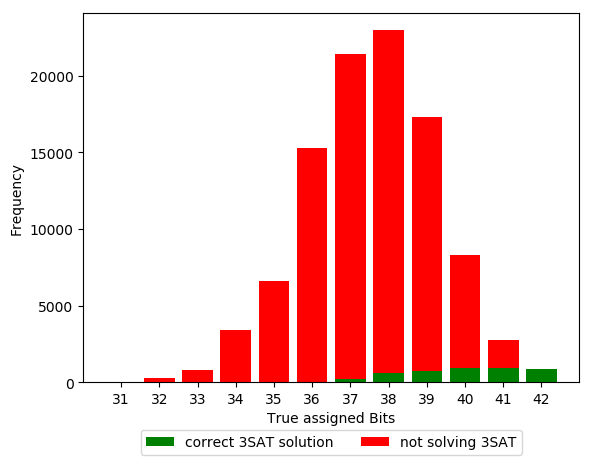
\includegraphics[width=.5\textwidth]{../material_2/Plots/42_4_2_def_engl_color_ohne_transform.png}%
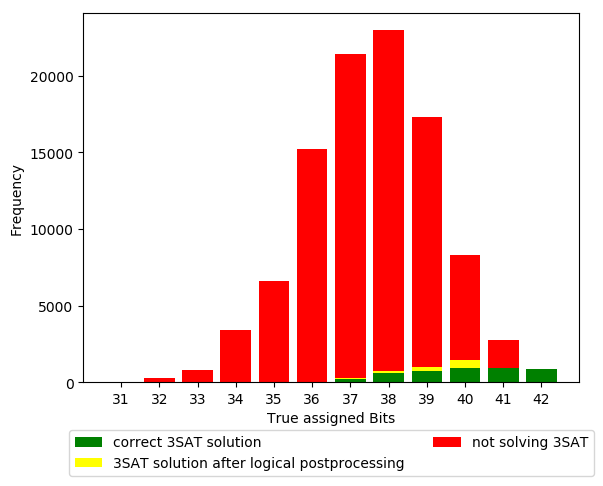
\includegraphics[width=.5\textwidth]{../material_2/Plots/42_4_2_def_engl_color_mit_transform.png}
\caption{Verteilung korrekter und nicht korrekter Antwortbitstrings ohne logisches Postprocessing (links) und mit logischem Postprocessing (rechts) für 3SAT-Instanzen bestehend aus 42 Klauseln und einem K/V- Verhältnis von 4,2.} \label{fig:distr}
\end{figure}

\begin{figure}
\centering
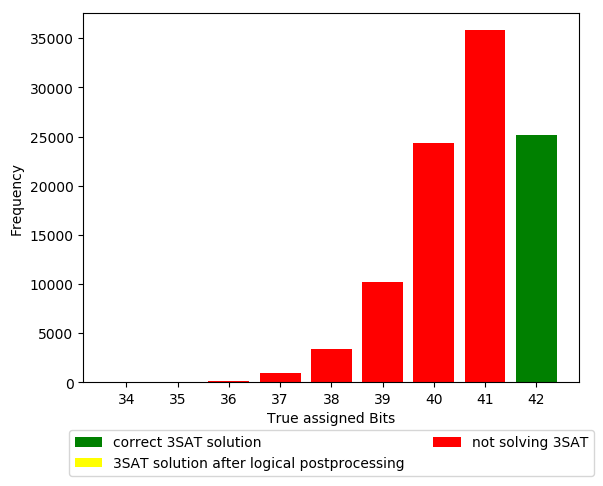
\includegraphics[width=.8\textwidth]{../material_2/Plots/42_4_2_opt_engl_color_mit_transform.png}
\caption{Verteilung korrekter und nicht korrekter Antwortbitstrings mit logischem Postprocessing für 3SAT-Instanzen bestehend aus 42 Klauseln und einem K/V- Verhältnis von 4,2.} \label{fig:distr}
\end{figure}

\begin{figure}
\centering
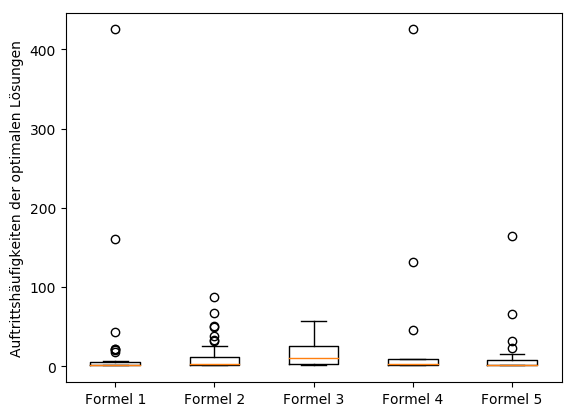
\includegraphics[width=.8\textwidth]{../material_2/25_clauses__4_2_def_MISBIAS.png}
\caption{Auftrittshäufigkeiten verschiedener optimaler Lösungen für verschiedene 3SAT-Formeln.} \label{fig:distr}
\end{figure}

\begin{figure}
\centering
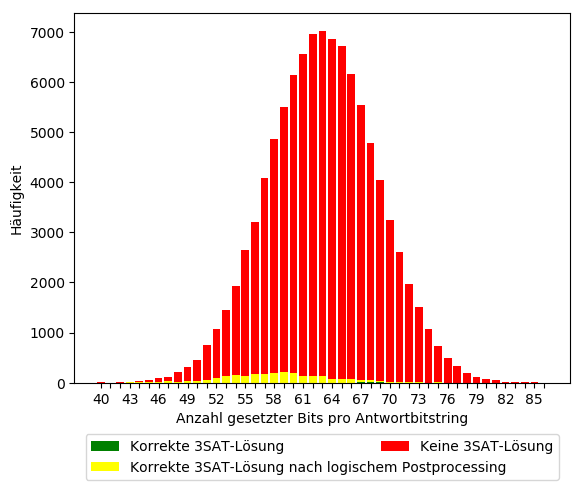
\includegraphics[width=.8\textwidth]{../material_2/42_clauses__0_2_def_RANDOM_color_transformed.png}%
%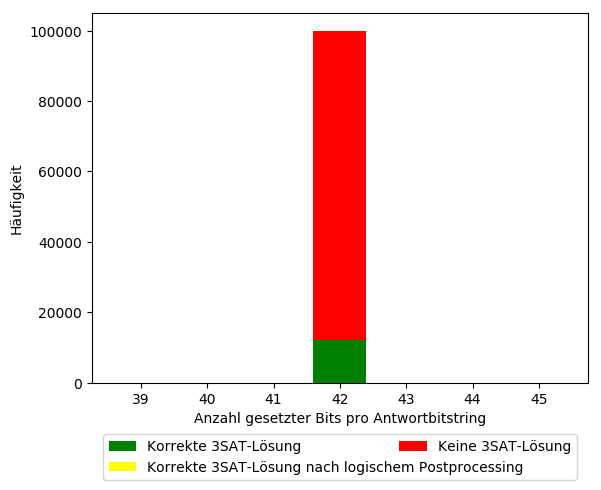
\includegraphics[width=.5\textwidth]{../material_2/42_clauses__0_2_def_RANDOM_CLEVER_color_transformed.png}
\caption{Verteilung korrekter 3SAT-Lösungen und falschen Antworten unter Ant- wortbitstrings, die durch den naiven Zufallsgenerator erzeugt wurden, mit bestimmter Anzahl gesetzter Bits für 3SAT-Formeln bestehend aus 42 Klauseln.} \label{fig:distr}
\end{figure}
